%%%%%%%%%%%%%%%%%%%%%%%%%%%%%%%%%%%%%%%%

\begin{frame}
\frametitle{Intuition}

$W$-parameterization learns everything from scratch

%Learning the Lakeland Terrier class from scratch is hard

\vspace{0.1in}
\begin{tabular}{m{0.7in}m{3.7in}}
    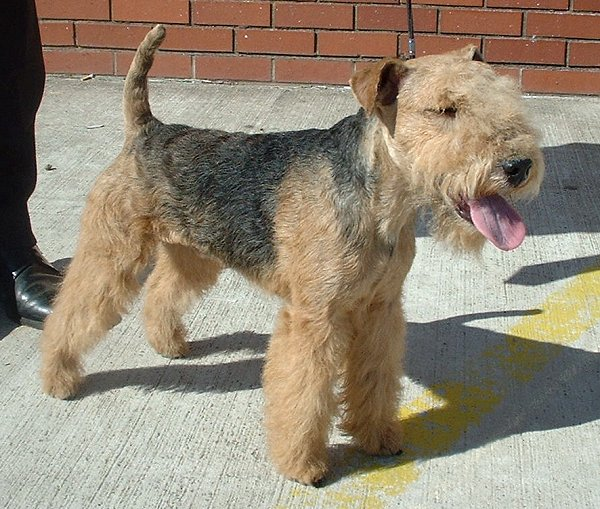
\includegraphics[height=0.5in]{img/Lakeland_Terrier} & How is \textbf{Lakeland Terrier} different than a tree? truck? person? horse? ... \\
    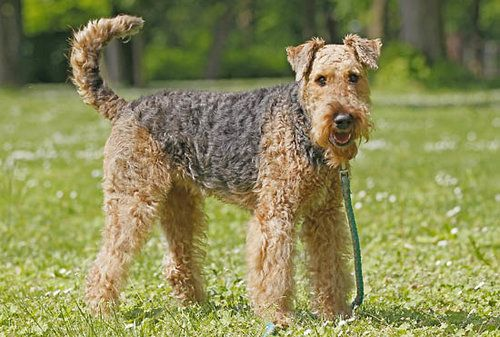
\includegraphics[height=0.5in]{img/Airedale} & How is \textbf{Airedale} different than a tree? truck? person? horse? ... \\
    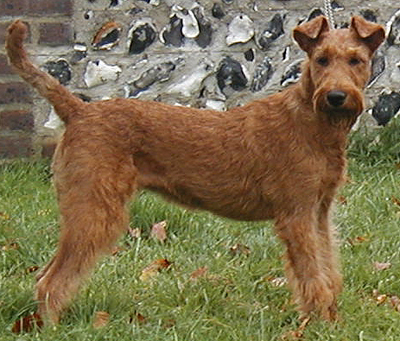
\includegraphics[height=0.5in]{img/Irish-Terrier} & How is \textbf{Irish Terrier} different than a tree? truck? person? horse? ... \\
    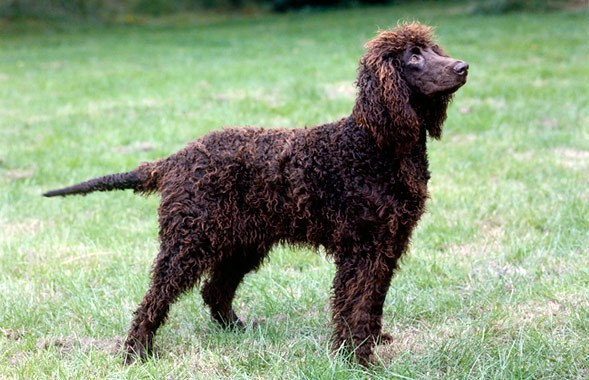
\includegraphics[height=0.5in]{img/water_spaniel} & How is \textbf{Irish Spaniel} different than a tree? truck? person? horse? ... \\
\end{tabular}
\end{frame}

\begin{frame}
\frametitle{Intuition}

$U$/$V$-tree parameterizations learn 1 class from scratch

\vspace{0.1in}
    \begin{tabular}{m{0.7in}m{3.8in}}
        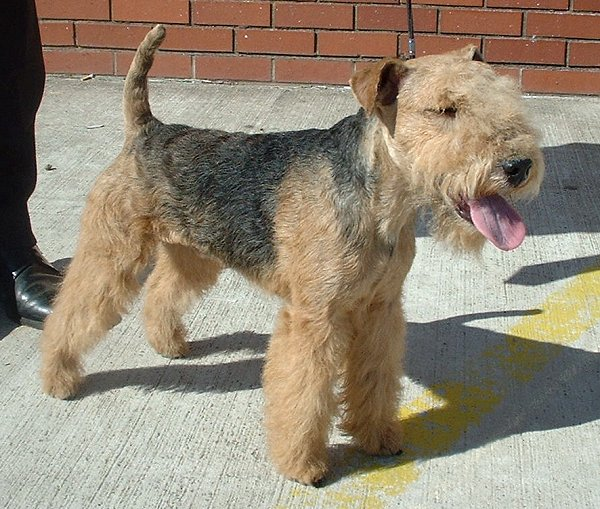
\includegraphics[height=0.5in]{img/Lakeland_Terrier} & How is \textbf{Lakeland Terrier} different than a tree? truck? person? horse? ... \\
\end{tabular}

\vspace{0.2in}
Learns only the difference between related classes

    \vspace{0.1in}
\begin{tabular}{m{0.7in}m{3.8in}}
    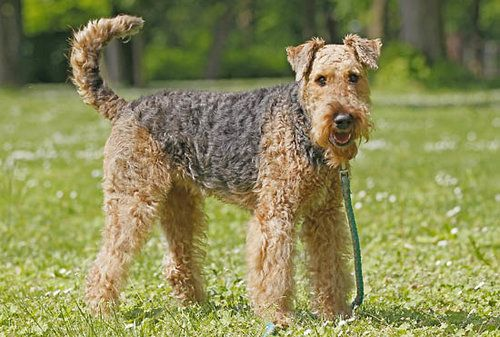
\includegraphics[height=0.5in]{img/Airedale} & \textbf{Airedale} is a big Lakeland Terrier \\
    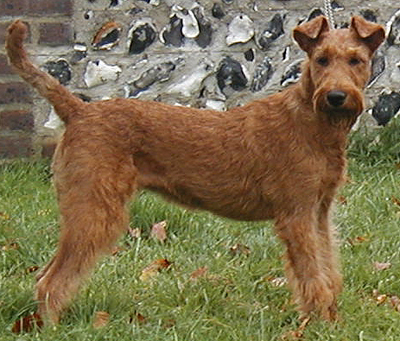
\includegraphics[height=0.5in]{img/Irish-Terrier} & \textbf{Irish Terrier} is a Lakeland Terrier with brown fur \\
    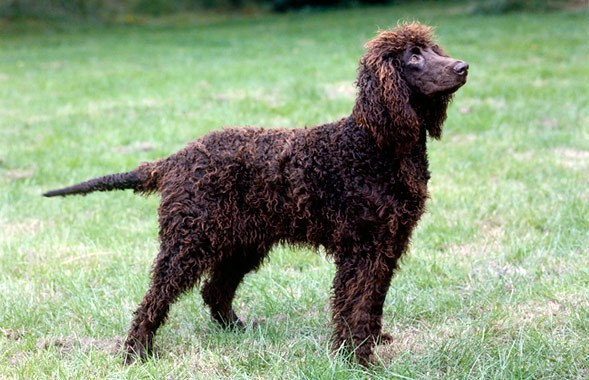
\includegraphics[height=0.5in]{img/water_spaniel} & \textbf{Irish Spaniel} is a Lakeland Terrier with long dark fur and big ears\\
\end{tabular}
\ignore{
\pause
    \vspace{0.3in}
Learn related classes by analogy (i.e.\ learn the difference)

    \vspace{0.1in}
\begin{tabular}{m{0.7in}m{3.8in}}
    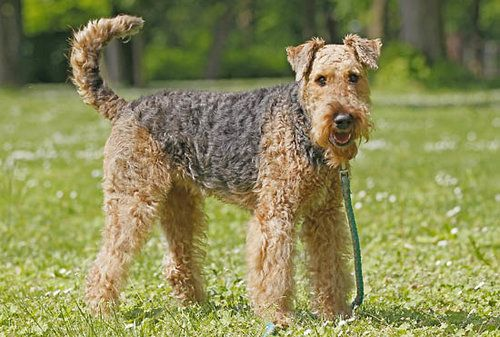
\includegraphics[height=0.5in]{img/Airedale} & Airedale is a big Lakeland Terrier \\
    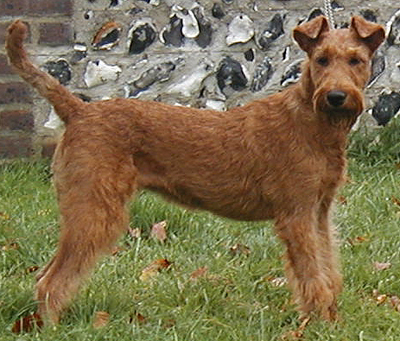
\includegraphics[height=0.5in]{img/Irish-Terrier} & Irish Terrier is a Lakeland Terrier with brown fur \\
    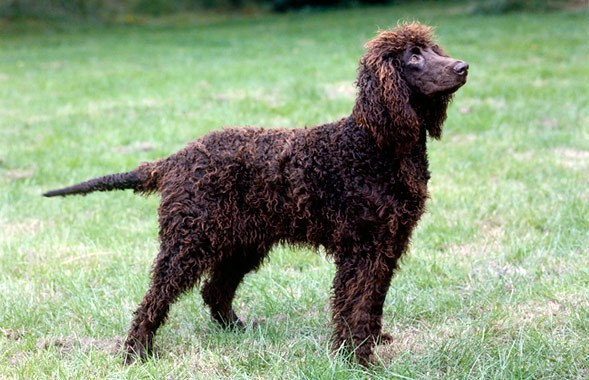
\includegraphics[height=0.5in]{img/water_spaniel} & Irish Spaniel is a Lakeland Terrier with long dark fur and big ears\\
\end{tabular}
}

\ignore{
Once I learn the ``concept'' of a Lakeland Terrier

    \begin{center}
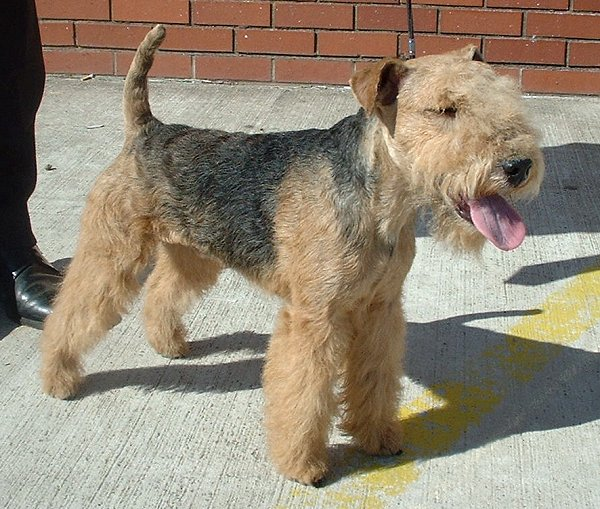
\includegraphics[height=1in]{img/Lakeland_Terrier}
    \end{center}

    \vspace{-0.1in}
    %\pause
I don't have to learn the concept of an Airdale from scratch

    \begin{center}
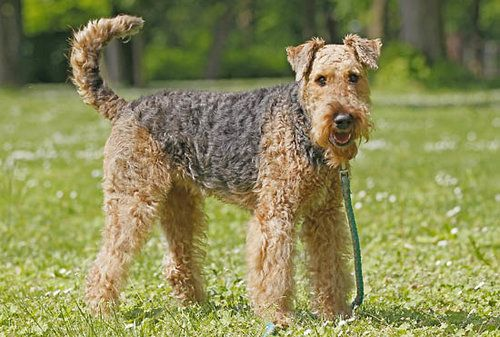
\includegraphics[height=1in]{img/Airedale}
    \end{center}

    \vspace{-0.1in}
I just learn the ``difference'' between these two classes
}

\end{frame}


